\subsection{Identifikation wesentlicher Energieeinsätze}

\subsubsection{Analyse und Unterscheidung von Energieeinsätzen}

Die DIN EN ISO 50001:2018-12 verpflichtet Organisationen im Rahmen der Planungsphase des PDCA-Zyklus zur Identifikation von wesentlichen Energieeinsätzen auf Grundlage 
der vorher durchgeführten Datenanalyse (\cite[S. 25]{DIN50001.2018}).
Die Norm definiert einen Energieeinsatz als Anwendung von Energie zum Beispiel für Energiedienstleistungen wie Lüftung oder Heizung, und bezeichnet den Begriff mitunter als 
Endnutzung von Energie (\cite[Kapitel 3.5.4]{DIN50001.2018}). 
Der Energieeinsatz ergibt sich aus dem Produkt des spezifischen Energieeinsatzes und der Menge der Nachgefragten Energiedienstleistungen (vgl. Gleichung \eqref{EnergieeinsatzMiller}) (\cite[S. 120]{Miller.2016}).
Der Spezifische Energieeinsatz ergibt sich aus dem Kehrwert der Energieeffizienz (vgl. Gleichung \eqref{EffizienzgleichungMiller}) (\cite[S. 120]{Miller.2016}).
\begin{equation}
    \text{Energieeinsatz} := \text{Spezifischer Energieeinsatz} \cdot \text{Menge Energiedienstleistung}
    \label{EnergieeinsatzMiller}
\end{equation}

\begin{equation}
    \text{Spezifischer Energieeinsatz} :=\frac{\text{Aufwand}}{\text{Erreichter Nutzen}}
    \label{SepzifischerEnergieinsatzMiller}
\end{equation}

Betrachtet man beispielsweise eine Heizungsanlage als nutzenseitige Energiedienstleistung im Untersuchungsgegenstand Gebäudezone.
So könnte man den erreichten Nutzen mit der Grundfläche konkretisieren. 
Der Aufwand wird durch den im Bilanzzeitraum anfallenden Nutzenergiebedarf zur befriedigung der Energiedienstleistung: Heizung gemessen.
Der Spezifische Energieeinsatz ist somit der im Bilanzzeitraum entstandene Nutzenergiebedarf zum Heizen pro Quadratmeter. 

Ein wesentlicher Energieeinsatz, auch SEU (en: significant energy use), wird von der Norm als Energieeinsatz der wesentlichen Anteil am Energieverbrauch 
hat und/oder erhebliches Potential für eine Verbesserung der energiebezogenen Leistung bietet definiert (\cite[Kapitel 3.5.6]{DIN50001.2018}). 
SEUs können Anlagen beziehungsweise Standorte, Systeme, Prozesse oder eine Einrichtungen sein (\cite[Kapitel 3.5.6]{DIN50001.2018}).
Zur Definition von Kriterien zur Identifikation von SEUs macht die Norm keine Angaben und verpflichtet die Organisation die die Norm anwendet zur Entscheidung was 
als wesentlicher Energieeinsatz anzusehen ist (\cite[S. 38]{DIN50001.2018}). 
Neben Energieerzeugungsanlagen und Umwandlungsanlagen gibt es Anlagenkategorien für Klimatisierungsanlagen, 
Lüftungsanlagen, Bleuchtungsanlagen sowie Informations- und Kommunikationstechnik (\cite[S. 14]{Hohnhold.2013}).

Eine differenzierte Darstellung der Verbrauchsstrukturen nach Anlagenkategorien beziehungsweise einzelner Anlagen ermöglicht das identifizieren von 
wesentlichen Energieeinsätzen und liefert somit auch Ansatzpunkte zur Verbesserung der Energieeffizienz (\cite{Fink.1997} zitiert nach \cite[S. 8]{Hohnhold.2013}).
Die in Abbildung \eqref{fig:Disagggregation_Bilanzraum_Nutzengrößen} dargestellte Disaggregation eines Bilanzraums nach Nutzengrößen kann bei der Analyse der 
Verbrauchsstrukturen innerhalb eines Untersuchungsgegenstands im Rahmen der Datenanalyse beitragen.



Abbildung \eqref{fig:Disagggregation_Bilanzraum_Nutzengrößen_Beispiel} zeigt Beispielhaft wie die Disagggregation von Bilanzräumen zur Identifikation von 
wesentlichen Energieeinsätzen beitragen kann. 
Der durch die aufwandsseitigen Ressourcen gedeckte Nutzenergiebedarf der bilanzierten Energiedienstleistung kann als absolute Energieleistungskennzahl zur 
Bewertung des Energieeinsatzes für die Energiedienstleistung betrachtet werden.
Der Energieeinsatz kann mit der durch die Bewertungseinheit quantifizierten Energiedienstleistung in relation gesetzt werden um den Spezifischen Energieeinsatz 
(vgl. Gleichung \eqref{SepzifischerEnergieinsatzMiller}) zu ermitteln, welcher als Beziehungszahl kategorisiert werden kann und somit geeignet zur Bewertung der Energieeffizienz ist. 
Die Integration einer Gliederungszahl als EnPI welche den Energieeinsatz eines Bilanzraums einer Energiedienstleistungen in Relation 
zum Energieeinsatz eines Bilanzraums aller Energiedienstleistungen setzt kann (vgl. Gleichung \eqref{Anteil_Gesamtenergieverbrauch}) den Vergleich des Anteils einzeln Energiedienstleistungen 
am Gesamtenergieverbrauch unterstützen.


\begin{equation}
    \text{Anteil Gesamtenergieverbrauch} :=\frac{\text{Energieverbrauch Bilanzraum}}{\text{Gesamtenergieverbrauch}}
    \label{Anteil_Gesamtenergieverbrauch}
\end{equation}

In diesem Beispiel macht die Heizungsanlage des Hauptgebäudes mit einem Energieeinsatz von 18.750 kWh 62,5 \% des Gesamtenergieverbrauchs aus und hat somit einen 
wesentlich Größeren Anteil am Gesamtenergieverbrauch als die Kühlungsanlage des Hauptgebäudes, welche mit einem Energieeinsatz von 3.750 kWh nur 12,5 \% des 
Gesamtenergieverbrauchs ausmacht.
Mit \( 125 \,\frac{\text{kWh}}{\text{m}^2} \) hat die Heizung den höchsten spezifischen Energieeinsatz und somit die geringst Energieeffizienz und die Kühlung 
mit \( 25 \,\frac{\text{kWh}}{\text{m}^2} \) den geringsten spezifischen Energieeinsatz und somit die höchste Energieeffizienz.

\begin{figure}[H]
    \centering
    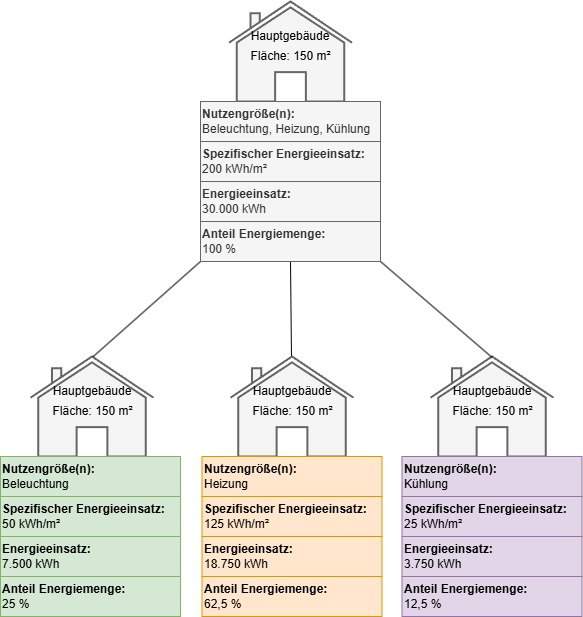
\includegraphics[width=0.7\textwidth]{../../Ressourcen/Abbildungen/Nutzengröße_Bewertungseinheit_Zerlegt_Beispiel.jpg}
    \caption{Beispiel: Disaggregation nach Nutzengrößen. (Eigene Darstellung)}
    \label{fig:Disagggregation_Bilanzraum_Nutzengrößen_Beispiel}
\end{figure}


Eine Analyse der Gebäudezonen innerhalb eines Gebäudes durch Disagggregation nach Untersuchungsgegenstand wie sie in 
\eqref{fig:Disagggregation_Bilanzraum_Untersuchungsgegenstand} visualisiert ist kann zur Identifikation wesentlicher Energieeinsätze durch die Analyse und Unterscheidung 
von Energieeinsätzen innerhalb von Gebäude(-zonen) beitragen.



Abbildung \eqref{fig:Disagggregation_Bilanzraum_Untersuchungsgegenstand_Beispiel} visualisiert beispielhaft, wie eine Disagggregation des Untersuchungsgegenstands 
zur Analyse und Unterscheidung von Energieeinsätzen innerhalb eines Untersuchungsgegenstands beitragen kann.
Zur Bewertung der einzelnen Bilanzräume werden die selben Energieleistungskennzahlen wie in Abbildung \eqref{fig:Disagggregation_Bilanzraum_Nutzengrößen_Beispiel} 
genutzt, allerdings wird der Bilanzraum anhand des Untersuchungsgegenstands disaggregiert.
In diesem Beispiel macht die Gebäudezone 2 mit einem Energieeinsatz von 18.000 kWh 60\% des Gesamtenergieverbrauchs des Gebäudes aus während Gebäudezone 3 mit 
einem Energieeinsatz von 3.000 kWh nur 10\% des Gesamtenergieverbrauchs ausmacht.
Der spezifische Energieeinsatz ist in Gebäudezone 2 mit  \( 300 \,\frac{\text{kWh}}{\text{m}^2} \) am höchsten und somit ist die Energieeffizienz am geringsten. 
In Gebäudezone 3 ist mit \( 100 \,\frac{\text{kWh}}{\text{m}^2} \) der spezifische Energieeinsatz am niedrigsten und die Energieeffizienz somit am höchsten.



\begin{figure}[H]
    \centering
    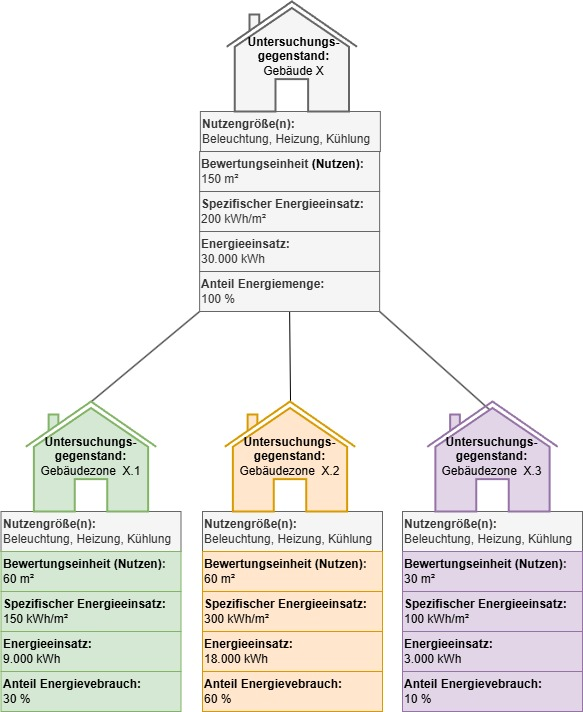
\includegraphics[width=0.7\textwidth]{../../Ressourcen/Abbildungen/Untersuchungsgegenstand_Zerlegt_Beispiel.jpg}
    \caption{Beispiel: Disaggregation nach Untersuchungsgegenstand. (Eigene Darstellung)}
    \label{fig:Disagggregation_Bilanzraum_Untersuchungsgegenstand_Beispiel}
\end{figure}